\chapter{The Array}
\label{chap:array}
\section{Why Arrays}

\begin{itemize}
	\item because new language: 
	Since this is a data structures course, I assumed that students have had exposure to arrays or array like objects.
	This chapter goes into a bit of a deeper detail that may have been glossed over and Introduces the topic in the appropriate language if need be.
	
	In other words, I assume you know what an array is , but not necessarily how to use it in Java or Python\footnote{Although we use lists in python}.
	\item  because internal memory lookup
	\item Because we need to make sure internal knowledge is cohesive (eg arrays of objects are arrays of pointers/references)
\end{itemize}







\section{Java and Arrays}
The Array is a built in class in Java, but the syntax is a bit unique \footnote{Enough so that I constantly had to look up how to do it my first two years of undergraduate studies, so don't feel too bad if you have to do the same.}

To create an array in Java we do:

\begin{minted}{Java}
	Type[] myArray = new Type[sizeOfArray]
\end{minted}


Here, every item in the array is of whatever \texttt{Type} we want, which could be a Class or primitive.   
Arrays can be whatever integer size we desire, but once set it cannot be changed.
This is because to create an array, the computer allocates a contiguous block of memory.
If we wanted to resize it, there is no guarantee that this chunk of memory won't have things directly before or after it, preventing us from safely extending its range.

\section{Python and Arrays}
\label{sec:python-arrays-lists}
Python doesn't really do arrays in the same way.
It instead uses Lists, as we'll see in Chapter \ref{chap:arraylist}.
\texttt{myNotArray = []}\footnote{On styles:  Java convention is to use camel case for variable types (\texttt{myVariableName}), while python convention is to use underscores (\texttt{my\_variable\_name}).  I will be using the Java style camel-casing for variables throughout the book for consistency and because it is my preference.}  does not actually make an array like you assume it would in some other language.  Instead it makes A list (specifically an array list ) to contain these items.
This works exactly like an array in other languages, but you get access to some nifty operations in Python, like slicing, concatination, and  built-in methods.  In addition, Python dynamically resizes this array if we need it bigger or smaller.\footnote{We cover the specifics in Chapter \ref{chap:arraylist}}



However, if you really want or need to use an array in python, you can.
%TODO factcheck
There are two ways to accomplish this.
The first way is the built in \texttt{array} package.  This builds a wrapper for the more primitive but efficient c-based array. 
The python package \texttt{numpy} contains yet \textit{another} type of array, this time much more focused on mathematical operations. 
In short, if you're working in python, use a list unless you know you should use something more specialized.







\section{How an Array Works}

As previously mentioned, an array creates a contiguous block of memory.  But what does this actually mean?
%autogenerated placeholder diagram  by chatgpt
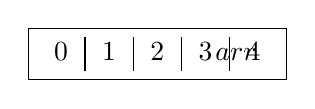
\begin{tikzpicture}
	\node[rectangle, draw] (array) {
		\begin{tabular}{c|c|c|c|c}
			0 & 1 & 2 & 3 & 4 \\
		\end{tabular}
	};
	\node[right of=array] (label) {$arr$};
\end{tikzpicture}

Here, $arr$ does not contain the array; it hold the memory location, the reference, the pointer to the array.  The correct term varies on the language you are using, but the point is that $arr$ tells you the location of the array rather than holding the array itself.


\subsection{Operations}

To review, arrays have two operations and one attribute: storing  a value at an index, retrieving a value from an index, and obtaining the size. 


For an array $arr$, retrieving a value from an array is and storing it in some variable is done with:

\begin{verbatim}
	myVar =  arr[index]
\end{verbatim}

and to store something in $arr$, you use:

\begin{verbatim}
	myVar = arr[index]
\end{verbatim}


Interestingly enough, this is one of the few consistent across multiple programming languages.

Figuring out the length of an array in Java\footnote{This is one of the little things in Java that can be a source of frustration.  Strings use \texttt{.length()}, arrays use \texttt{.length}, and Collections like Lists and Sets use \texttt{.size()}.} is done with \mintinline{Java}{arr.length;}, 
and in python, a simple \mintinline{Python3}{len(arr)} works.

%\begin{minted}{Java}
%	int len = arr.length;
%\end{minted}


\subsection{Array Internals and the Memory Formula}
\label{array-formula}


So how does an array actually work?  How do you actually retrieve a value from an index?
The most crucial thing to keep in mind in this textbook is when you see something like the code below:
\begin{verbatim}
	variable = expression;
\end{verbatim}

The left side is always a variable.  The expression on the right side always\footnote{except for primitives, like \texttt{int} in Java} yields some memory location.  This means you should repeat to yourself ``the memory location on the right gets stored in the variable on the left.''

This means that 
\begin{minted}{Java}
	int[] numbers = new int[10];
\end{minted}

stores a memory location in \texttt{numbers}.  It does not store 10 integers in \texttt{numbers}.  It only tells you where to find them.  Specifically, it stores the memory location of index 0 of the array.  This is true for not only Java, but C as well, and almost every programming language\footnote{Python and other interpreted languages are slightly more complicated because we are dealing with array lists, thus one additional level of abstraction, so this storage just happens a layer deeper.  Esoteric languages like \textit{ook} and \textit{Malbolge}  prevent me from making a statement like ``all languages.'' }. 


This means that 

What if we aren't dealing with primitives, but with objects like Strings instead?  
In this case, each slot in the array doesn't hold the object itself but instead \textit{a reference to that object}.
Thus, each slot needs to be big enough to hold a memory address, ie 32 bits or 64 bits depending on the machine.





\section{Common Array Algorithms}

\subsection{Finding Values in an Array}
\subsubsection{Finding the Minimum}

Hopefully you know this one by now!
Simply assume the first item is the smallest item, then check it against every other item in the array.  If an item is smaller that the current smallest item, it replaces the smallest item.

\begin{javacode}[listing and comment, comment={As seen in the comments, it is fairly straightforward to change this code to return the index, rather than the item.}]{Finding the Minimum of An Array}
public static int findMin(int[] arr) {
	int smallest = arr[0];
	// int smallestIndex = 0;
	for (int i = 1; i < arr.length; i++) {
		if(arr[i] < smallest){
			smallest = arr[i];
			// int smallestIndex = i;
		}
	}
	return smallest; // or smallestIndex
}
\end{javacode}



\subsubsection{Finding the Average}


\subsection{Limitations}
Arrays are awesome solutions for many problems, but they are lacking in ability for some problems.  Consider the following exercise:

\begin{verbatim}
	
	Given a string of text, determine what the most common character of text is. 
	
\end{verbatim}
Unless you've seen this problem before, there is no obvious solution.  Considerable thought eventually lands on an idea: characters are just integers, so we could assign each one of the characters an index and increment the index each time we see the character.

\begin{javacode}{Most Frequent ASCII Character}
public static char mostFrequent(String text) {
	int[] tally = new int[128]; 
	for(char c : text.toCharArray()) {
		tally[(int) c] += 1;
	}
	
	indexWithHighest = 0;
	for(int index = 0; index<128; index++) {
		if( tally[index] > tally[indexWithHighest]){
			indexWithHighest = index;
		}
	}
	return (char) indexWithHighest;
}

\end{javacode}


However, this has some serious limitations.  For one, this breaks if we are not using ascii.  What if the text is ``こんにちは'' or other non-english text? 
You could create a larger array for all 100000+ unicode characters, but this begins to become less and less feasible.  
And now what if we change the problem to:

\begin{verbatim}
	
	Given a string of text, determine what the most common word is. 
	
\end{verbatim}

This suddenly becomes an extremely annoying problem to solve with just arrays\footnote{Those of you coming from Python can stop shouting ``use dictionaries!'' at the top of your lungs.}.  We will solve this problem when we visit Maps in Chapter \ref{chap:maps}, which are much better suited for this job than arrays.

The other limitation of arrays that their size is immutable.  Once an array has been declared, we cannot change its size.  This is rather inconvenient for a number of applications where we may not know how many items to store.  This will be the focus of our first new data structure:  The List.


